%%%%%%%%%%%%%%%%%%%%%%%%%%%%%%%%%%%%%%%%%%%%%%%%%%%%%
\chapter{Formulation as an Optimal Transport Problem}
The Damped Newton algorithm developed by M\'{e}rigot et al. \cite{Merigot2017} solves a semi-discrete Monge-Amp\`{e}re type optimal transport problem. It's efficiency in exploiting the properties of sparse matrices and linear convergence \cite{Merigot2017} make it practical for implementation in the solution for equations \ref{EadyGC}. Further detail describing the application of the algorithm in the solution to the Eady Model is given in chapter \ref{algorithm}. In this chapter an overview of semi-discrete optimal transport is given using definitions given in \cite{Kitagawa2016, Merigot2017} as well as a comparison to the energy minimisation to which it is applied. A rigorous proof of the formulation of \ref{EadyModel} as a Monge-Amp\`{e}re type optimal transport problem is given in Cullen, 2006 \cite{Cullen2006a}.
\section{Semi-discrete Optimal Transport}
\begin{figure}[h]
	\centering
	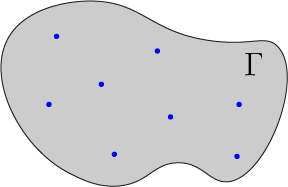
\includegraphics[width=5.5cm]{project/probmeasure}
	\caption[Semi-discrete Optimal Transport]{A discrete (target) set $Y \subseteq \mathbb{R}^2$ represented by blue points in a compact domain (source) $\Gamma \subseteq \mathbb{R}^2 $}
	\label{fig:probmeasure}
\end{figure}
Optimal transport problems describe the problem of finding a map between two sets, each with an associated density, in such a way that the "cost" associated with the mapping is minimised. In semi-discrete optimal transport the target set is a finite set.\\
\linebreak
In Kitagawa et al. \cite{Kitagawa2016} a wonderful analogy with travel distance to bakeries in a city is made. The example considers a population in the city and a finite set of locations of bakeries in the city. It is assumed that the population is uniformly distributed in the city. The optimal transport problem finds a partition of the city such that every point in a region of the partion is closest to the bakery at the centre of that region. In this analogy the cost being minimised is the travel distance to the bakery $c(\bm{x},\bm{y}_i) = \|\bm{x}-\bm{y}_i \|^2$. This is illustrated in figure \ref{fig:laguerrediagram0w}  below
\begin{figure}[h]
	\centering
	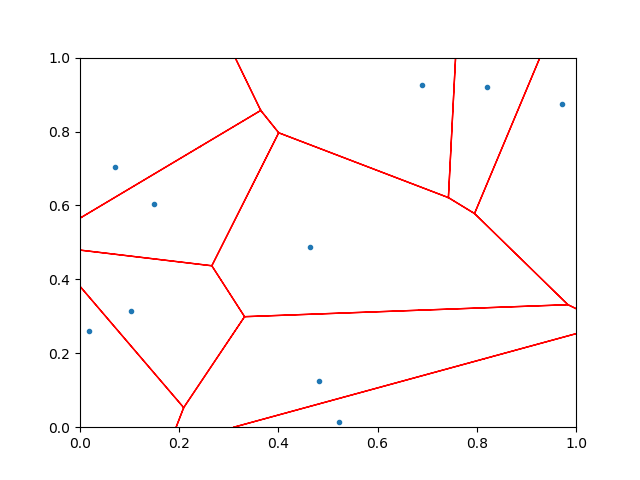
\includegraphics[width=7cm]{project/laguerre_diagram_0w}
	\caption[The partitioning of a city]{The image showing how a city would be divided into areas based on minimising distance to the local bakeries denoted by blue points}
	\label{fig:laguerrediagram0w}
\end{figure}
\\
To put this into a more rigorous mathematical setting, given a domain  $\Gamma\subseteq \mathbb{R}^2$ and discrete set of $N$ points $Y = \left\lbrace \bm{y}_i, \quad 1\leq i \leq N \right\rbrace  \subset \mathbb{R}^2$,\\
\linebreak
\textbf{Source measure} $\mu(A) = \int_A \rho(x)dx$, $A \subseteq \Gamma$ with $\rho$ a probability density on $\Gamma$\\
The \textbf{Target measure} $\nu = \sum_{1\leq i \leq N}\nu_i \delta_{y_i}$, with finite support on $\mathbb{R}^2$, where $\nu_i \in \mathbb{R}$ and $\delta_{y_i}$ is the delta function centred at the point $\bm{y}_i$\\
\linebreak
The partition of the city is described mathematically by \textbf{Voronoi Cells} \\ $\text{Vor}_y := \left\lbrace x \in \Gamma \; \text{st} \; \forall z \in Y \; c(x,y) \leq c(x,z) \right\rbrace$\\
\linebreak
Following \cite{Kitagawa2016} we then define a \textbf{Transport map}, $T: \Gamma \rightarrow Y$ between the source measure $\mu$ and the target measure on $Y$, $\mu$ if $T_{\#}\mu = \nu$.\\
\linebreak
The \textbf{Pushforward} of a measure $\mu$ by a map $T: \Gamma \rightarrow Y$ is $T_{\#}\mu = \sum_{\bm{y}_i \in Y} \mu \left( T^{-1}(\bm{y}_i) \right) \delta_{\bm{y}_i}$, the sum of the measures of the set mapped to the point $\bm{y}_i$ under $T$
\\
From these definitions we can see that the optimal transport map is given by,
\begin{equation}
	T(x) = \arg\min_{y\in Y}\left(c(x,y)\right)
\end{equation}
or equivalently if 
\begin{equation}
\nu_i = \mu\left(\text{Vor}_{y_i}\right)
\end{equation}
Figure \ref{fig:laguerrediagram0w} above shows the Voronoi diagram for the example of bakeries in a city
\comments{not sure about this section - also a lot of it is paraphrased from the \cite{Kitagawa2016} paper}
\section{Laguerre Cells and the Inclusion of weights}
 \begin{figure}[h]
	\centering
	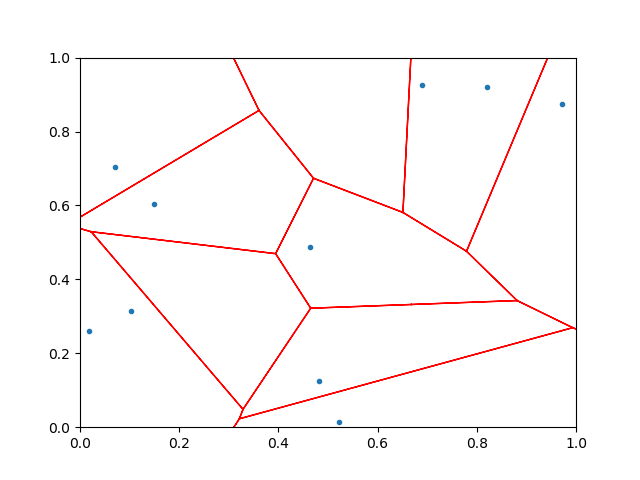
\includegraphics[width=7cm]{project/laguerre_diagram_OTw}
	\caption[Laguerre diagram produced by finding weights using damped newton algorithm for optimal transport]{Given a uniform source and target density the Laguerre diagram produced by finding weights using damped newton algorithm for optimal transport}
	\label{fig:laguerrediagramotw}
\end{figure}
Considering again the example of bakeries in the city, looking at figure \ref{fig:laguerrediagram0w} it is clear that if the population density across city is uniform the distribution of customers to each bakery is certainly not. For example, the Voronoi cell at the centre of the diagram is much larger in area than those in the top right of the diagram. This raises the problem of finding a way to create a partion so that each cell has the same area. This is done by introducing an additional \textquotedblleft weight \textquotedblright  argument to the cost. We denote the weights by $\psi_i = \psi\left(\bm{y}_i\right)$. In the case of the bakeries the weights might represent the price of bread at a specific bakery. For example in figure \ref{fig:laguerrediagram0w} if the bakery at the centre charged more for bread the population living on the outskirts of the cell would be more incentivised to travel further for cheaper bread.\\
\linebreak
The cells are now called  \textbf{Laguerre Cells}, defined as \\ $\text{Lag}_{y_i}(\psi) := \left\lbrace x \in K \; \text{st} \; \forall y_j \in Y \; c(x,y) + \psi(y_i) \leq c(x,z) + \psi(y_j) \right\rbrace$ \\ 
\linebreak 
In this case, the optimal transport map is given by \\
$T_\psi: x \rightarrow \text{argmin}_i\| x - y_i \|^2 + \psi_i$, where $\psi_i = \psi(y_i)$ is a family of weights on $Y$ \cite{Merigot2017}.\\
\linebreak
 The problem is then finding the weights $\psi_i$ associated to the points $y_i$ such that $G_i(\psi) := \mu (\text{Lag}_{y_i}(\psi)) = \nu_i$. The Damped Newton's Algorithm from M\'{e}rigot, Meyron and Thibert (2017) \cite{Merigot2017} finds such $\psi_i$.
 \\
 \linebreak 
 Supposing that both the source density and target density are uniform, the Laguerre cells as found by the code developed in \cite{Merigot2017} are show in figure \ref{fig:laguerrediagramotw}. The cells in this case are the Laguerre cells defined above, and the optimal transport map was found by \cite{Merigot2017} as
 \begin{equation*}
 T(x) = \arg\min_{y\in Y}\left(c(x,y) + \psi_i(y)\right)
 \end{equation*}
For the remainder of this report we will consider cases where both the source density and target density are uniform and the quadratic cost function
\begin{equation*}
	c(x,y) = \| x - y \|^2
\end{equation*}
\section{Applying semi-discrete optimal transport to solving the semi-geostrophic equations}
As shown in \cite{Cullen2006a} equations \ref{EadyModel} can be recast as an optimal transport problem using the transformation to geostrophic co-ordinates introduced by Hoskins \cite{Hoskins1975}. In this section we outline how the damped newton algorithm is applied to equations \ref{EadyModel}.
\\
\linebreak
The optimal transport problem considered in the frontogenesis problem is the minimisation of the energy, restated from equation \ref{energy}
\begin{equation}
E = f^2 \iint \frac{1}{2}\left(X-x\right)^2 - Z\left(z - H/2\right)\textrm{d}x\textrm{d}z
\end{equation}
as show in section \ref{Geostrophic} this is equivalent to minimising \ref{energy1}
\begin{equation}
E = \frac{f^2}{2} \iint \left(\left(X-x\right)^2 + \left(Z - z\right)^2\right)\textrm{d}x\textrm{d}z
\end{equation}
Considering the geostrophic co-ordinates as the target set of finite set of points for the optimal transport problem from the domain $\Gamma = [-L,L] \times [0,H]$. The Damped Newton Algorithm finds the weights such that the area of each Laguerre cell is preserved.
\section{Extension for Periodic Boundary Conditions}
As stated in Chapter \ref{governingequations} in the model for frontogenesis boundary conditions consider periodicity in $x$. This must be accounted for in the implementation of the Damped Newton Algorithm.
\\
\linebreak
This inclusion of periodic boundary conditions means that Laguerre cells may cover areas over the right and left boundaries. This means that the Laguerre edges must be continuous across the boundaries if copies of the Laguerre diagram were placed on each boundary. As well as all the Laguerre cells must have the same mass. This is illustrated in the Laguerre diagram in figure \comments{insert periodic Laguerre diagram and explain}
A detailed explanation of how this was implemented for solving the semi-geostrophic equations is included in section \ref{timestep}.\\
\linebreak
\comments{include the definition of mass of a cell and a better written description of the partion given by a laguerre diagram (tesselation/zero measure sets)}

%%%%%%%%%%%%%%%%%%%%%%%%%%%%%%%%%%%%%%%%%%%%%%%%%%%%%
\chapter{A Numerical Solution to the Eady Model for Frontogenesis \label{algorithm}}
In this section the numerical implementation including the use of the Damped Newton Algroithm developed by \cite{Merigot2017} is explained in detail. 
Restating the problem, we are solving the semi-geostrophic equations \ref{EadyModel} over the domain $\Gamma := [-L,L] \times [0,H]$.
\begin{equation*}
	\begin{aligned}
		-fv_g + \frac{\partial \varphi}{\partial x} = 0,\\
		\frac{Dv_g}{Dt} + fu -\frac{Cg}{\theta _0}\left(z-H/2\right) = 0,\\
		\frac{D\theta'}{Dt} - Cv_g = 0,\\
		\frac{\partial \varphi}{\partial z} - g\frac{\theta'}{\theta_0} = 0,\\
		\nabla \cdot \bm{u} = 0.
	\end{aligned}
\end{equation*}
With boundary conditions:
\vspace{-\topsep}
\begin{itemize}
	\setlength{\parskip}{0pt}
	\setlength{\itemsep}{0pt}
	\item Rigid lid condition $w = 0$ on $z = 0, H$
	\item Periodic boundary conditions in $x$
\end{itemize}
\vspace{-\topsep}
Together with a baroclinic instability described by \ref{thetap} as
\begin{equation}
\theta' = \frac{N^2\theta_0 z}{g} + B\sin\left(\pi\left(x/L + z/H\right)\right)
\end{equation}
The steps involved in solving the Eady Model for frontogenesis described above are detailed below,
\begin{description}
	\setlength{\parskip}{0pt}
	\setlength{\itemsep}{0pt}
	\item[Step 1] Initialise a set of physical points in space
	\item[Step 2] Transform physical points to Geostrophic space using the co-ordinate transformation given in \ref{Geostrophic}
	\item[Step 3] Given the points in geostrophic space the weights which define the Laguerre cells in the physical domain are calculated using the Damped Newton Algorithm.
	\item[Step 4] The equations are now time stepped from the transformed momentum equations \ref{EadyGC} 
	\begin{equation*}
		\begin{aligned}
			\frac{\mathrm{D}X_{n}}{\mathrm{D}t} -\frac{Cg}{f\theta _0}\left(\tilde{z}_n-H/2\right) = 0 \\
			\frac{\mathrm{D}Z_{n}}{\mathrm{D}t} - \frac{Cg}{f\theta_0}\left(X_n - \tilde{x}_n\right) = 0
		\end{aligned}
	\end{equation*}
	Where $X_n, Z_n$ represent the geostrophic points at the current time step, and $\tilde{x}_n,\tilde{z}_n$ represent the centroids of the Laguerre cells. In this project both a Forward-Euler scheme and Heun's method have been used for time-stepping.
	\item[Step 5] The geostrophic points are now replaced with $X_{n+1}, Z_{n+1}$ and steps 3 and 4 are repeated until the final time is reached.
\end{description}
\comments{include pseudocode overview??}
\section{Initialisation of Points in Geostrophic Space \label{Initpoints}}
Given a finite set of equidistant points in the physical domain $\Gamma$, the points are transformed to geostrophic space using
\begin{equation}
X = x + \frac{v_g}{f}, \qquad Z = \frac{g\theta'}{f^2\theta_0}
\label{geostrophictransformation}
\end{equation}
This requires the form of $\theta'$ given by \ref{thetap} from this $v_g$ can be deduced using the following equations from \ref{EadyModel},
\begin{equation}
	\begin{aligned}
		\frac{\partial \varphi}{\partial z} - \frac{g \theta'}{\theta_0} = 0\\
		\frac{\partial \varphi}{\partial x} - fv_g = 0
	\end{aligned}
\label{findingvg}
\end{equation}
using the boundary condition $\int_{0}^{H}\varphi(x,z)\text{ d}z = 0$
Integrating the first equation in $z$,
\begin{equation*}
	\begin{aligned}
	\frac{\partial \varphi}{\partial z} = \frac{g \theta'}{\theta_0} = N_0^2z + \frac{Bg}{\theta_0}\sin\left(\pi\left(\frac{x}{L}+\frac{z}{H}\right) \right)\\
	\varphi = \frac{N_0^2z^2}{2} - \frac{BgH}{\theta_0\pi}\cos\left(\pi\left(\frac{x}{L}+\frac{z}{H}\right)\right) + F(x)
	\end{aligned}
\end{equation*}
Applying the boundary condition to determine $F(x)$,
\begin{equation*}
	\begin{aligned}
	\int_{0}^{H}\varphi \text{ d}z = \left[ \frac{N_0^2z^3}{6} -`  \frac{BgH^2}{\theta_0\pi^2}\sin\left(\pi\left(\frac{x}{L}+\frac{z}{H}\right) \right) + F(x)z\right]_{0}^{H} = 0
	\end{aligned}
\end{equation*}
Using $\sin\left(\frac{\pi x}{L}+\pi\right) = -\sin\left(\frac{\pi x}{L}\right)$,
\begin{equation*}
\begin{aligned}
 0 & =\frac{N_0^2H^3}{6} - \frac{BgH^2}{\theta_0\pi^2}\sin\left(\frac{\pi x}{L}+\pi\right)+ \frac{BgH^2}{\theta_0\pi^2}\sin\left(\frac{\pi x}{L}\right) + F(x)H\\
 0 & =\frac{N_0^2H^3}{6} + \frac{2BgH^2}{\theta_0\pi^2}\sin\left(\frac{\pi x}{L}\right) + F(x)H
\end{aligned}
\end{equation*}
This gives $F(x)$ as,
\begin{equation*}
	F(x) = -\frac{N_0^2H^2}{6} - \frac{2BgH^2}{\theta_0\pi^2}\sin\left(\frac{\pi x}{L}\right)
\end{equation*}
and consequently $\varphi$ as,
\begin{equation}
	\varphi(x,z) = \frac{N_0^2z^2}{2} - \frac{BgH}{\theta_0\pi}\cos\left(\pi\left(\frac{x}{L}+\frac{z}{H}\right)\right)-\frac{N_0^2H^2}{6} - \frac{2BgH}{\theta_0\pi^2}\sin\left(\frac{\pi x}{L}\right)
\end{equation}
Using the second of equations \ref{findingvg} $v_g$ is found as,
\begin{equation}
	v_g = \frac{BgH}{f\theta_0L}\cos\left(\pi\left(\frac{x}{L}+\frac{z}{H}\right)\right)- \frac{2BgH}{f\theta_0\pi}\sin\left(\frac{\pi x}{L}\right)
\end{equation}
Together with $\theta'$ given by \ref{thetap} this expression for $v_g$ can be used to determine $X$ and $Z$ in geostrophic co-ordinates through the transform \ref{geostrophictransformation}.
\comments{Image of transformed points??}
\section{Choice of Initial Weights \label{Initweights}}
The Laguerre diagram of this set of points shown in figure \comments{insert image showing geostrophic points + reference to image} with zero weights would define Laguerre cells exterior to $\Gamma$. These cells will have zero \textquotedblleft mass \textquotedblright in the domain $\Gamma$. Physical intuition tells us that given the rigid lid and periodic boundary conditions points would physically not be able to leave the domain. However, thinking of fluid particles as the centroids of Laguerre cells, a cell outside the domain would represent a fluid particle on the exterior of the domain. This also poses a problem with respect to the implementation of the Damped Newton Algorithm, as emphasised in \cite{Merigot2017}, as it requires $\mu\left(\text{Lag}_{y_i}(\psi)\right)$ to be a monotonic function of $\psi = (\psi(y_1),...,\psi(y_N))$ where $N$ is the number of points initialised in $\Gamma$. According to \cite{Merigot2017} this occurs near points where the Laguerre cells contain positive mass over $\Gamma$.\\
\linebreak
Fortunately, a solution is provided in \cite{Merigot2017}. Proposition 25 in the paper proves that if the initial weights are given by,
\begin{equation*}
	\psi_i^0 = d\left(\bm{Y}_i,\Gamma\right)^2
\end{equation*}
where $\bm{Y}_i = \left(X_i,Z_i\right)$ are the points in geostrophic space. Since the domain is rectangular vertical distance from the point to the upper or lower boundary of the domain. The boundaries, given by $z=0$ and $z = H$ are also perturbed to guarantee strict positivity of the mass of the Laguerre cells, 
\begin{equation*}
\psi_i^0 = \begin{cases}
\left(Z_i - 0.9H\right)^2, & Z_i > 0.9H \\
\left(Z_i - 0.1H\right)^2, & Z_i < 0.1H
\end{cases}
\label{weights}
\end{equation*}
\comments{Address disparity with paper '-' sign - convention used in paper for finding laguerre cells different to code?}
The Damped newton algorithm is initialised with the the geostrophic points and weights given by \ref{weights}. The algorithm outputs weights that give Laguerre cells with equal mass over the periodic domain.
\section{Time Stepping \label{timestep}}
\subsection{Forward-Euler Scheme}
The numerical solution to equations \ref{EadyModel} developed follows a Lagrangian framework, thus it is justified to treat the material derivative $\frac{\mathrm{D } }{\mathrm{D} t}$ as the usual $\frac{\mathrm{d }}{\mathrm{d} t}$, in this sense we will develop prognostic scheme using the equations,
	\begin{equation*}
	\begin{aligned}
	\frac{\mathrm{d}X}{\mathrm{d}t} -\frac{Cg}{f\theta _0}\left(\tilde{z}-H/2\right) = 0 \\
	\frac{\mathrm{d}Z}{\mathrm{d}t} - \frac{Cg}{f\theta_0}\left(X - \tilde{x}\right) = 0
	\end{aligned}
	\end{equation*}
Applying a Forward-Euler scheme for time-stepping given by,
\begin{equation}
	\begin{aligned}
	t_i^{n+1} &= t_i^n + h\\
	Z_i^{n+1} &= Z_i^n + \frac{hCg}{f\theta_0}\left(X_i^n-\tilde{x}_i^n\right)\\
	X_i^{n+1} &= X_i^n + \frac{hCg}{f\theta_0}\left(\tilde{z}_i^n-H/2\right)
	\end{aligned}
\end{equation}
where $\tilde{x}_i^n,\tilde{z}_i^n$ represent the centroids of the Laguerre cells given by $X_i^n,Z_i^n$ and corresponding weights given by the optimal transport algorithm,
\begin{equation}
	\tilde{x}_i^n = \frac{\int_{\mathrm{Lag}_{Y_i^n}(\psi)} x \mathrm{d}x \mathrm{d}z}{\int_{\mathrm{Lag}_{Y_i^n}(\psi)} \mathrm{d}x \mathrm{d}z}, \qquad
	\tilde{z}_i^n = \frac{\int_{\mathrm{Lag}_{Y_i^n}(\psi)} z \mathrm{d}x \mathrm{d}z}{\int_{\mathrm{Lag}_{Y_i^n}(\psi)} \mathrm{d}x \mathrm{d}z}
\end{equation}
Before the next iteration of the time-step the points $X_i^{n+1}, Z_i^{n+1}$ are mapped back to the fundamental domain.
\subsection{Heun's Method}

\comments{include map back to fundamental domain explanation and why this isn't done for centroids}

\section{Visualising the Output \label{plotting}}

%%%%%%%%%%%%%%%%%%%%%%%%%%%%%%%%%%%%%%%%%%%%%%%%%%%%%
\chapter{Unsorted}
\section{Linear Stability Analysis}
Starting from the Eady Model \ref{EadyModel} restated below
\begin{equation}
	\begin{aligned}
	-fv_g + \frac{\partial \varphi}{\partial x} = 0,\\
	\frac{Dv_g}{Dt} + fu -\frac{Cg}{\theta _0}\left(z-H/2\right) = 0,\\
	\frac{D\theta'}{Dt} - Cv_g = 0,\\
	\frac{\partial \varphi}{\partial z} - g\frac{\theta'}{\theta_0} = 0,\\
	\nabla \cdot \bm{u} = 0.
	\end{aligned}
\label{EadyModel2}
\end{equation} 
Linearise about a base state given by Hoskins \cite{Hoskins1975},
\begin{equation}
	\begin{aligned}
		\bar{\theta} &= \theta_0 \frac{N_0^2\theta_0 z}{g} - Cy \\
		\bar{\varphi} &= \theta_0 + \frac{N_0^2 z^2}{2}\\
		\bar{v}_g &= 0\\
		\bar{U} &= \frac{Cg}{f\theta_0}\left(z - H/2\right)\\
		\bar{W} &= 0 
	\end{aligned}
\end{equation}
Introduce a perturbation and linearise about base state,\\
$u = \bar{U} + u'$, $w = w'$, $v_g =  v_g'$, $\varphi = \bar{\varphi} + \varphi'$, $\theta ' = \bar{\theta} + \theta ''$\\
Introducing the stream function,
\begin{equation}
	u' = \frac{\partial \psi}{\partial z},\qquad w' = -\frac{\partial \psi}{\partial x} 
\end{equation}
Looking for normal modes solutions of the form,
\begin{equation*}
	q' = \hat{q}(z)\exp^{i \left(kx - \omega t\right)}
\end{equation*}
Equations \ref{EadyModel2} become,
\begin{align}
 		-f\hat{v}_g + ik\hat{\varphi} = 0,\label{stab1}\\
 	-i\omega \hat{v}_g + ik\bar{U}\hat{v}_g + f\frac{\text{d}\hat{\psi}}{\text{d}z} = 0,\label{stab2}\\
 	-i \omega \hat{\theta} + i k \bar{U} \hat{\theta} - ik\frac{N_0^2\theta_0}{g} \hat{\psi} - C\hat{v}_g = 0,\label{stab3}\\
 	\frac{\text{d}\hat{\varphi}}{\text{d}z} - g\frac{\hat{\theta}}{\theta_0} = 0 \label{stab4},
\end{align}
First eliminating, $\varphi$, equations \ref{stab1} and \ref{stab4} give,
\begin{equation*}
	-f\frac{\text{d}\hat{v}_g}{\text{d}z}+ik\frac{\text{d}\hat{\varphi}}{\text{d}z} = 0, \qquad \frac{\text{d}\hat{\varphi}}{\text{d}z} - g\frac{\hat{\theta}}{\theta_0} = 0
\end{equation*}
so that,
\begin{equation}
	\hat{\theta} = \frac{f\theta_0}{ikg} \frac{\text{d}\hat{v}_g}{\text{d}z}
\label{thetahat}
\end{equation}
Rearranging equation \ref{stab3}
\begin{equation}
	 i\left( k \bar{U} - \omega \right) \hat{\theta} - ik\frac{N_0^2\theta_0}{g} \hat{\psi} - C\hat{v}_g = 0
\label{stab3.1}
\end{equation}
Eliminating $\hat{\theta}$ using \ref{thetahat}
\begin{equation*}
	\frac{f\theta_0}{kg}\left( k \bar{U} - \omega \right)  \frac{\text{d}\hat{v}_g}{\text{d}z} - ik\frac{N_0^2\theta_0}{g} \hat{\psi} - C\hat{v}_g = 0
\end{equation*}
from equation \ref{stab2} we have
\begin{equation}
	i\left( k \bar{U} - \omega \right) \hat{v}_g - f \frac{\text{d}\hat{\psi}}{\text{d}z} = 0
\label{stab2.1}
\end{equation}
differentiating this expression we find
\begin{equation*}
	ik \frac{\text{d}\bar{U}}{\text{d}z} \hat{v}_g + i(k\bar{U}-\omega)\frac{\text{d}\hat{v}_g}{\text{d}z} + f\frac{\text{d}^2{\psi}}{\text{d}z^2} = 0 
\end{equation*}
Substituting this expression with \ref{stab2.1} into \ref{stab3.1}, noting that,
\begin{equation*}
	(k\bar{U}-\omega)\frac{\text{d}\hat{v}_g}{\text{d}z} = if\frac{\text{d}^2{\psi}}{\text{d}z^2} + \frac{fk}{i(k\bar{U}-\omega)}\frac{\text{d}\bar{U}}{\text{d}z}\frac{\text{d}\hat{\psi}}{\text{d}z}
\end{equation*}
\begin{equation*}
	\frac{f\theta_0}{kg}\left(if\frac{\text{d}^2{\psi}}{\text{d}z^2} + \frac{fk}{i(k\bar{U}-\omega)}\frac{\text{d}\bar{U}}{\text{d}z}\frac{\text{d}\hat{\psi}}{\text{d}z}\right) - \frac{ik N_0^2\theta_0\hat{\psi}}{g} + \frac{Cf}{i(k\bar{U}-\omega)}\frac{\text{d}\psi}{\text{d}z} =0
\end{equation*}
Rearranging gives,
\begin{equation*}
	-\frac{f^2\theta_0}{kg}(k\bar{U}-\omega)\frac{\text{d}^2{\psi}}{\text{d}z^2}+\left(Cf+\frac{f^2\theta_0}{g}\frac{\text{d}\bar{U}}{\text{d}z}\right)\frac{\text{d}\hat{\psi}}{\text{d}z}+\frac{k N_0^2\theta_0}{g}(k\bar{U}-\omega)\hat{\psi}=0
\end{equation*}
\begin{equation*}
	-f^2\theta_0(k\bar{U}-\omega)\frac{\text{d}^2{\psi}}{\text{d}z^2}+2Cfkg\frac{\text{d}\hat{\psi}}{\text{d}z}+k^2 N_0^2\theta_0(k\bar{U}-\omega)\hat{\psi}=0
\end{equation*}
We reformulate this as a matrix eigenvalue problem for $\omega$
\begin{equation}
	-f^2\theta_0\bar{U}\frac{\text{d}^2{\psi}}{\text{d}z^2}+2Cfkg\frac{\text{d}\hat{\psi}}{\text{d}z}+k^2 N_0^2\theta_0\bar{U}\hat{\psi}=\omega \left(k^2N_0^2\theta_0\hat{\psi}-f^2\theta_0 \frac{\text{d}^2{\psi}}{\text{d}z^2}\right)
\label{stabanalysis}
\end{equation}
Introducing a second order finite difference scheme for $\psi$
\begin{equation*}
	\begin{aligned}
	\frac{\text{d}^2{\hat{\psi}}}{\text{d}z^2} = \frac{\psi_{i-1} - 2\psi_i + \psi_{i+1}}{h^2}\\
	\frac{\text{d}\hat{\psi}}{\text{d}z} = \frac{\psi_{i-1} - \psi_{i+1}}{2h}
	\end{aligned}
\end{equation*}
Equation \ref{stabanalysis} becomes
\begin{equation}
	\begin{aligned}
	-f^2\theta_0\bar{U}_i\left(\frac{\psi_{i-1} - 2\psi_i + \psi_{i+1}}{h^2}\right)+2Cfkg\left(\frac{\psi_{i-1} -f \psi_{i+1}}{2h}\right)+k^3 N_0^2\theta_0\bar{U}_i\psi_i= \\
	\omega\left(k^2N_0^2\theta_0\psi_i-f^2\theta_0\left(\frac{\psi_{i-1} - 2\psi_i + \psi_{i+1}}{h^2}\right)\right)
	\end{aligned}
\end{equation}
Discretising the interval $[0,H]$ into $N$ points with step size $h$ we can recast this as an eigenvalue problem,
\begin{equation*}
	A\bm{\psi} = \omega B\bm{\psi}
\end{equation*}
to find eigenvalues $\omega$ with corresponding eigenvectors $\bm{\psi} = \left(\psi_1, ... , \psi_{N-2}\right)$. Since the boundary condition gives $\psi = 0$ on $z = 0, H$, $\psi_0 = \psi_N = 0$ so these are omitted from the $\hat{\phi}$ vector but considered in the finite difference schemes for $\psi_1$ and $\psi_{N-1}$
The coefficients matrix $A$ are given by
\begin{equation}
	\begin{aligned}
		\psi_{i-1}:& \quad -\frac{-f^2\theta_0k\bar{U}_i}{h^2} - \frac{Cfkg}{h}\\
		\psi_i:& \quad \frac{2f^2\theta_0k\bar{U}_i}{h^2} + k^3N_0^2\theta_0\bar{U}_i\\
		\psi_{i+1}:& \quad \frac{-f^2\theta_0k\bar{U}_i}{h^2} + \frac{Cfkg}{h}\\
	\end{aligned}
\end{equation}
$i: 1 \rightarrow N-2$ with $\psi_0 = \psi_{N}$. The coefficients of matrix $B$ are given by,
\begin{equation*}
	\begin{aligned}
		\psi_{i-1}:& \quad -\frac{f^2\theta_0}{h^2}\\
		\psi_i:& \quad k^2N_0^2\theta_0 + \frac{2f^2\theta_0}{h^2}\\
		\psi_{i+1}:& \quad -\frac{f^2\theta_0}{h^2}\\
	\end{aligned}
\end{equation*}
\begin{figure}[h]
	\centering
	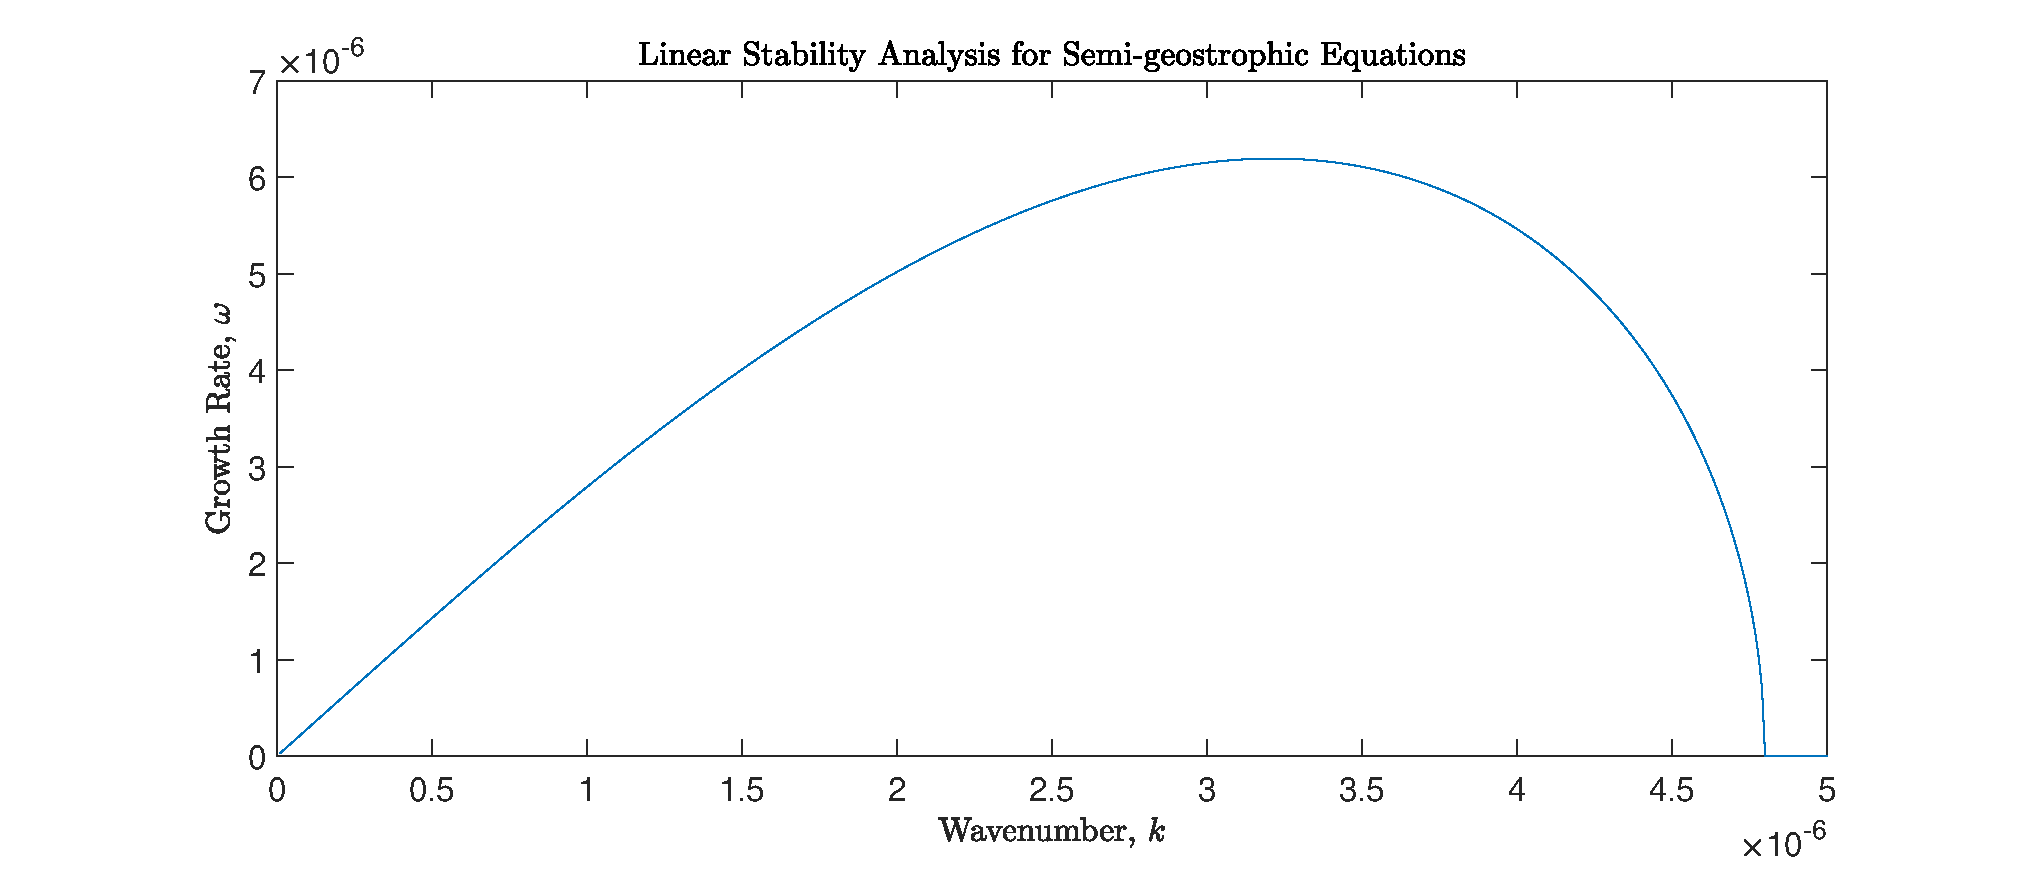
\includegraphics[width=\linewidth]{project/Linear_stability_analysis}
	\caption[Linear stability analysis results for the semi-geostrophic equations]{Plot showing growth rate, $\omega$ against wavenumber $k$ for the Eady model of the semi-geostrophic equations}
	\label{fig:linearstabilityanalysis}
\end{figure}
\section{Calculation of Moments applying periodic boundary conditions}